\section{MAX-MIN}
\subsection{TÓM TẮT LÝ THUYẾT}
Cho hàm số $y=f(x)$ xác định trên tập $\mathscr{D}$. Ta có
\immini{\begin{itemize}
        \item $M$ là giá trị lớn nhất của hàm số nếu $\heva{&f(x) \le M,\forall x \in \mathscr{D}\\& \exists x_0 \in \mathscr{D}: f(x_0)=M.}$\\
        Kí hiệu \fbox{$\displaystyle\max_{x \in \mathscr{D}}f(x)=M$}
        \vskip 0.5cm
        \item  $m$ là giá trị nhỏ nhất của hàm số nếu $\heva{&f(x) \ge m,\forall x \in \mathscr{D}\\& \exists x_0 \in \mathscr{D}: f(x_0)=m.}$\\
        Kí hiệu \fbox{$\displaystyle\min_{x \in \mathscr{D}}f(x)=m$}
    \end{itemize}
}{
    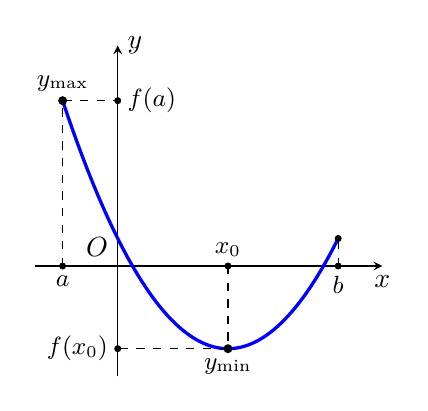
\begin{tikzpicture}[smooth,samples=300,scale=0.7,>=stealth]
        \draw[->] (-1.5,0)--(4.8,0) node[below]{$x$};
        \draw[->] (0,-2)--(0,4) node[right]{$y$};
        \draw (0,0) node[above left]{$O$};
        \draw[line width = 1.2pt,domain=-1:4,blue] plot(\x,{0.5*((\x)^2-4*(\x)+1)});
        \draw[fill=black] (-1,0) circle(1.5pt) (-1,3) circle(2pt) (0,3) circle(1.5pt) (0,-1.5) circle(1.5pt) (2,0) circle(1.5pt) (2,-1.5) circle(2pt) (4,0) circle(1.5pt) (4,0.5) circle(1.5pt);
        \draw[dashed] (-1,0)node[below]{\small$a$}--(-1,3)--(0,3)node[right]{\small$f(a)$} (2,0)node[above]{\small$x_0$}--(2,-1.5)--(0,-1.5)node[left]{\small$f(x_0)$}
        (4,0)node[below]{\small$b$}--(4,0.5);
        \node[above] at (-1,3) {\small $y_{\max}$};
        \node[below] at (2,-1.5) {\small $y_{\min}$};
\end{tikzpicture}}
\begin{note}
    Khi yêu cầu tìm max min của hàm số mà không nói rõ xét trên tập nào, thì ta hiểu là tìm max min trên miền xác định của hàm số đó.
\end{note}
